%%% Architecture section

\section{Monitoring Architecture}
There are many proposed architectures for use in runtime monitoring. Fundamental questions such as where the monitor executes (\eg`, external hardware or on-system), what the monitor watches (\eg, memory values, executed instructions, etc.) and how the monitor obtains input (\eg, system instrumentation, external sensors) are dependent on both the properties of the system being monitored and the desired effects of monitoring (\ie, observation or enforcement/control).  

Existing runtime monitoring techniques tend to clash with the constraints imposed by safety-critical embedded systems. 
Many existing monitors rely on automatic generation of instrumentation code or generation of the monitor itself (\eg, \cite{Havelund2004, Pike2011}).
This is unusable with black-box components or external supplier scenarios due to the lack of source code access. They also have have a greater chance of affecting the non-faulty system behavior, especially timing in real-time systems.
Instead, we propose a passive external monitor which only checks system properties that are observable by passively observing system state from an existing broadcast bus.
%These include not only direct constraints including cost sensitivity and real-time computation but also development constraints such as system certification and source code access for black-box components.
We focus on ground vehicles and CAN buses specifically in this work, but other similar systems and broadcast networks can also be monitored using this approach.
%Although we focus on ground vehicles and CAN in this work, other similar systems can also be monitored with this approach due to the flexible interface and system model.
For example, systems without a broadcast bus may be monitored by exposing the desired system state to the monitor (either through instrumentation or intelligent monitor placement such as network gateways/routers).

\subsection{Architecture Outline}
An outline of our monitor architecture is shown in Figure \ref{fig:architecture}. 
The monitor is connected to the target system as an additional passive node on its broadcast bus. 
The monitor's \textsf{SF Map} generates the system trace by building the necessary propositions based on the observed bus traffic. 
%
%This bus is connected to the system interface which observes the bus traffic and generates the system trace for the monitor. The interface builds the trace by periodically creating the set of atomic propositions which make up the trace state. 
%This bus is connected to the system interface which observes the bus traffic and generates the atomic propositions for the monitor based on the observed bus state, building a system state snapshot for the monitor. 
%The trace that is formally monitored is a series of these snapshots. 
This generated trace is provided to the monitoring algorithm which checks it against the given system specification, outputting whether the trace violated or satisfied the specification at each trace step (subject to delays waiting on future trace state).
The algorithm's output is sent to an action controller which can perform the desired response to any specification violations, such as logging the violations or triggering a recovery action.

%The target system is monitored by filtering the observable system state through a semi-formal mapping which produces the system trace $\sigma$. 
%This trace, along with the desired system specification $\varphi$ is provided to the formal monitoring algorithm \agmon\ which outputs whether the system trace satisfies or violates the given specification. This output can then be used to trigger a warning or perform some other recovery action as desired.

\begin{figure}
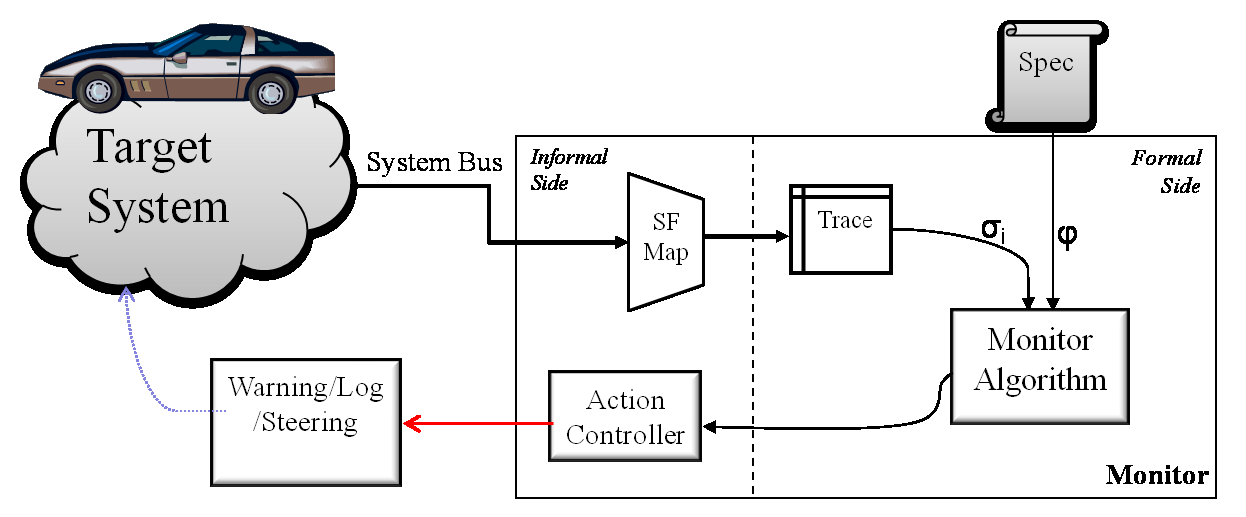
\includegraphics[width=4.5in]{img/mon_arch}
\caption{External monitor architecture outline \label{fig:architecture}}
\end{figure}

This architecture separates the lower-level system dependent configuration from the high-level system specification in a way similar to MaC \cite{Kim2004}.
%This architecture separates the system-independent formal aspects of the monitor from the system-dependent components including the system interface and action controller. 
%By utilizing a semi-formal interface, we can separate the formal aspects of the monitor, which are completely independent from the target system, from the more practical pieces: the monitor interfaces and their configurations, which are system dependent. 
This allows us to utilize a core formal monitoring algorithm and framework with any system where an \textsf{SF Map} can be used to create a system trace.
Separating the system dependent and system-independent aspects of the monitor also lets the high level system requirements be somewhat abstracted away from the implementation. This means that changes to the target system may only require changes to the interface configuration and not the high level system specification. 
%This is a similar situation to the two-level specifications used in the MaC framework \cite{Kim2004}.

\subsection{System Interface}
Different systems have varying specification needs which can not always be easily met within a formal specification language. 
In order to provide flexibility to map system state onto the formal specification language (in our case, in propositions) we provide a \textsf{SF Map} interface which defines the mapping between the observed system state and the monitored specification. 
This type of interface is common in monitors for real systems, including MaC's filters \cite{Kim2004} and the AP evaluation filter from \cite{Heffernan2014}.
